%\documentclass[draftclsnofoot,onecolumn]{IEEEtran}
\documentclass[3p]{elsarticle}
\usepackage{tipa}
\usepackage{amsmath}%math
\usepackage{amsthm}%proof
\usepackage{xcolor}%color
\usepackage{bm}
\usepackage{graphicx}
\usepackage{booktabs}
\usepackage{textcomp}
\usepackage[colorlinks,linkcolor=black,anchorcolor=black,citecolor=black]{hyperref}
\usepackage{amsfonts,amssymb}
\usepackage{color,soul}
\theoremstyle{plain}
\newtheorem{myas}{Assumption}
\newtheorem{mydef}{Definition}
\newtheorem{mylem}{Lemma}
\newtheorem{mythm}{Theorem}
\newtheorem{mypro}{Properties}
%\theoremstyle{remark}
\theoremstyle{remark}
\newtheorem{myrem}{Remark}
\begin{document}
\begin{frontmatter}
\title{Dynamic Adaptive Saturated Sliding Mode Control For Deployment of Tethered Satellite System}
\author{Zhiqiang Ma}
\author{Guanghui Sun\corref{cor1}}
{\author{Zhengkai Li\corref{cor2}}}
\ead{guanghuisun@hit.edu.cn}
\cortext[cor1]{Corresponding author}
\address{Research Institute of Intelligent Control and Systems, Harbin Institute of Technology, Harbin 150001, China}



\begin{abstract}
This paper presents a novel adaptive dynamic sliding mode scheme for the deployment of the tethered satellite system. The tethered satellite system is modelled based on Lagrangian mechanics theory, and to overcome the limited input of the dynamic model, a new scalable dimensionless transform and strictly bounded terms are designed to guarantee the existence of the ratio between limited input and command signal. The adaptive saturated sliding mode control scheme is proposed to govern the tether deployment by introducing the adaptive rate into the system gain, and the stability analysis indicates that this measure can eliminate the uncertainty caused by the input limitation to guarantee that the asymptotically stability of the deployment dynamics. The numerical simulations are reported to verify the effectiveness of the proposed control laws.
\end{abstract}
\begin{keyword}
Tethered satellite;  Sliding mode control;  Input limitation; Adaptive control
\end{keyword}
\end{frontmatter}
\section{Introduction}
The deployment is the key technology of the space tethered satellite system~\cite{wen2008advances,yousefian2015anti}, and this technique supports various applications for space exploration and scientific research, such as space debris removal~\cite{zhao2014thrust}, space elevator~\cite{kojima2015mission}, satellite de-orbit~\cite{zhong2013dynamics,zhong2013long} and the tethered space robot~\cite{huang2014optimal}. Many international space research institutes have launched some orbital, suborbital and ground experiments in an effort, such as TSS-1R, SEDS, MAST and YES2, to verify the feasibility of the proposed theoretical and simulation design for the deployment of the tethered satellite system~\cite{williams2012review,robitaille2006interpreting,stone1998tss,williams2009yes2}. These experimental results make researchers proceed to advance mechanics, kinetic and control studies intensively, to tackle the challenges of requirements from space missions in the future~\cite{yu2016nonlinear,wen2015space,aslanov2016swing,meng2016lyapunov,zhang2015line}.\par

Recent scientific researches on deployment of the tethered satellite focus on the stabilization of the dynamics, and have varying merit and outcomes, providing different kinds of control schemes, including tension, thruster, electrodynamic and Coulomb approach~\cite{kojima2015stabilisation,qi2016dynamics,zhong2016research}. Among the deployment stabilization strategies, the hybrid tension and thruster control boosts to the new developments. Iki et al. implemented the ground experiment of an electrodynamic tether deployment from a spool-type reel, and the thruster was used to guarantee the deployment of kilometers-length space tether~\cite{iki2014experiments}. Aslanov et al. presented a thruster method driving the space tethered tug, and analyzed the dragging dynamics~\cite{aslanov2013dynamics}. Huang et al. investigated the attitude and deploying dynamics of the tethered space robot from the standpoint of thruster consumption~\cite{huang2015coupling}. Jung et al. adopted thruster scheme to achieve the ideal deployment rate during the deployment of three-body tethered satellites~\cite{jung2015nonlinear}. Liu et al. equipped the thruster system, which consisted of four pairs of thrusters, in the subsatellite dedicating for regulation of the attitude and deployment dynamics~\cite{liu2014attitude}. Zakrzhevskii divided the deployment process into two stages, the first stage of which ejected the tether with thruster to position the tether at desired beginning point of the second stage, and the second stage continued to adjust the tether to the stable vertical configuration by using tension generated by friction~\cite{zakrzhevskii2016method}. Mantellato et al. reported the thrust-aided librating deployment of tape tethers, and the force acting on the tape tether included the tension and thruster force~\cite{mantellato2015thrust}. This hybrid strategy has several advantages, such as simplifying the input model greatly, non-environmental dependence (magnetic field dependence), easy assembly and physical implementation, thus is broadly utilized in reality compared with other control strategies.\par

There also exist some obstacles in the design of the hybrid control. Particularly, it's a prime problem that tension actuators and thrusters are both constrained by physical and chemical condition, i.e., the tether is not available to be repressed like the stick, and meanwhile too big tether length rate might break the space tether. Also, the thruster can not provide infinite force~\cite{martinez1998spacecraft}. Hence the tension and thruster force for the deployment/retrevial are both limited, and in the view of control theory, the phenomena usually causes the input limitation of a dynamic system. Substituting limited inputs into unmodified conventional control scheme designed for unlimited input system results in lost of control or poor performance, and theoretically, such kind of implement is unreasonable. Hence to cope with input limitation in the tethered satellite system (TSS), some scientific researchers spent much effort on restricting input, providing many solutions on satellite arrangements and deployments. Huang et al. addressed an adaptive postcapture backstepping control of the tethered space robot, and analyzed the effect of constrained input by using specific auxiliary design systems~\cite{huang2015adaptive}. Wen et al. took into account the positive bounded tension constraint by designing the feedback control with special saturation technique~\cite{wen2016constrained}, and Wen also proposed some remarkable achievements using optimal control for deployment~\cite{wen2008optimal}. Liu et al. reported the variable structure scheme for the deployment with thruster control, where the thruster is used to guarantee the positive tension during the mission~\cite{yingying2012variable}. In summary, existed studies deal with the major issue about the deployment with restricted tension and thruster force in two ways, accordingly, the suitable physical compensation and the elaborate design of limited input. In aspect of designing elaborate limited inputs, as Wen et al. explained, the limited terms, including the tension and the state of the deployment, can be viewed as the solution of a nonlinear optimal control \cite{wen2015tension}. Hu reported an adaptive sliding mode control with saturated input by using reduced sliding dynamic design approach \cite{Hu2009Robust}, which requires an assumption that the command signal is bounded strictly, and for actual physical systems, this assumption always exits. In this paper, a new dynamic adaptive saturated sliding mode  control for the deployment of the tethered satellite system is studied. For coping with the input saturation in the hybrid control strategy, the strictly saturated command signal is constructed with Sine saturation function. Based on the feature of the saturated command, an adaptive rate is introduced into the controller design to remove the effect of the input limitation theoretically. In order to improve the performance of the sliding phase, the terminal attractor is incorporated into the design of the ideal sliding surface. Numerical simulations are performed to illustrate that the stabilization of the deployment is accomplished by the controller designed in spite of the input limitation.\par
The paper is organized as follows: Section \ref{sec:2} introduces the standard mathematical model of the deployment of the TSS. Section \ref{sec:3} designs the adaptive saturated sliding mode control laws with input limitation for the dynamics, and these simulations are exhibited in Section \ref{sec:4} to reveal the effectiveness and efficiency. The conclusion is given in Section \ref{sec:5}.
\section{Mathematical model}\label{sec:2}
Figure \ref{fig:1} shows all the elements of the TSS via the geometric representation. In the figure, it is apparent that $OXYZ$ denotes the inertial frame, the origin $O$ of which is arranged at the the earth's core. $OX$ and $OY$ are mutually perpendicular axes on the equatorial plane with $OX$ pointing to the spring equinox, and $OZ$ is perpendicular to the equatorial plane, bundling the axis of the earth upwards. The frame of $OXYZ$ fulfills the right-hand rule, hence the direction of axis $OY$ is identified. Orbital coordinate system is denoted as $O_2xyz$ with the origin $O_2$ located at the center of the TSS. $O_2x$ points to the orbital direction, meanwhile $O_2z$ is along the direction downwards towards to the core of the earth, generating the axis $O_2y$ by utilizing the right-hand rule. $\theta$ and $\phi$ stand for the in-plane and out-of-plane angle, respectively. Another coordinate system $O_2x'y'z'$ represents the TSS frame with $O_2z'$ pointing to the subsatellite along the tether, and $O_2x'y'z'$ can be obtained by rotating $O_2xyz$ around the fixed origin $O_2$. $\bm R_0$ denotes the position vector between $O_2$ and $O$.\par
In the analysis of the deployment of the TSS, there is a primary assumption that the movement of entire system is approximating to a ``rolling ball'' behavior with three DOFs modelled, and reasonably one can invoke the spherical coordinates to describe the behavior. During space mission, the mass of the tether is much smaller than that of the mother satellite, and hence it is always ignored sufficiently. Some other assumptions are obvious throughout the analysis, and listed in the following. A satellite is able to be regard as a particle under the condition that the length of the tether is large enough, and due to the tiny ratio of the mass between the satellites, the deployment of the subsatellite will not effect the motion of the mother satellite and keep the nominal orbit during the whole mission. The deployment is regulated by the tension and thrusters, and to guarantee the establishment of the ``rolling ball'' model, the tether remains inextensible, straight and stiff all the time.\par
Before giving out the model, some preliminary symbols are exhibited. $R_0$ is a positive scaler meaning the radius of orbit without disturbance, and $\Omega = \sqrt{\mu_e/R_0^3}$ is the orbital angular velocity where $\mu_e$ is the coefficient of the Earth gravity field.\par
Based on the assumption above, the kinetic energy and the potential energy of the deployment dynamics can be described as:
\begin{figure}[http]
\centering
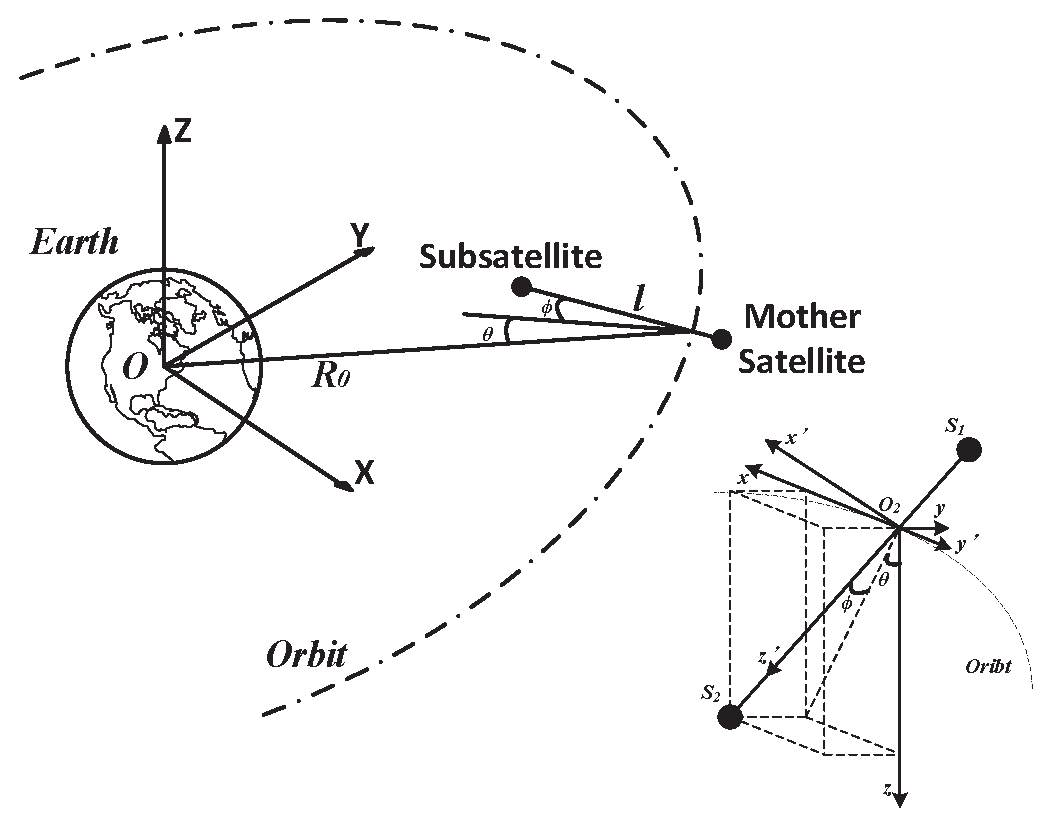
\includegraphics[width=0.7\textwidth]{paper4_fig1.eps}
\caption{TSS geometric representation}
\label{fig:1}
\end{figure}
\begin{align}
T_t
&= \frac{1}{2}\sum\limits_{s=1}^2 m_s\bm{R_s'\cdot R_s'}\notag\\
&= \frac{1}{2}m\bm{R_0'\cdot R_0'}+\frac{1}{2}\sum\limits_{s=1}^2 m_s\bm{r_s'\cdot r_s'}\notag\\
&= \frac{1}{2}m\Omega^2R_0^2+\frac{1}{2}\bar{m}l^2\begin{bmatrix}\phi'+(\theta'+\Omega)^2\end{bmatrix}+\frac{1}{2}\bar{m}l'^2\label{eq:Tt1}\\
V_g
&= -\mu_e\sum\limits_{s=1}^2\frac{m_s}{\vert \bm{R_0+r_s}\vert}\notag\\
&= -m\Omega^2R_0^2+\frac{\bar{m}\Omega^2l^2}{2}(1-3\cos{^2\theta}\cos^2\phi),\label{eq:Vg}
\end{align}
where, $m = m_1+m_2$ stands for the total mass of the system, $m_1$ and $m_2$ of which denote the mass of the mother satellite and of the subsatellite, respectively. $(\cdot)'$ represents the differentiation with respective to time, and $l$ means the tether length connecting the satellites. $\theta$ and $\phi$ depict the rolling and pitching dynamics of the TSS. For clarity, $m_1m_2/m$ is rewritten as $\bar m$.
Combining Eq.~(\ref{eq:Vg}) and Eq.~(\ref{eq:Tt1}) give rise to the Lagrange function:
\begin{align}
\begin{split}
L=&T_t-V_g\\
=&\frac{\bar ml^2}{2}\begin{pmatrix}\phi'^{2}+\cos^2\phi(\theta'+\Omega)^2\end{pmatrix}+\frac{\bar ml'^2}{2}\\
&-\frac{\bar m\Omega^2l^2}{2}\begin{pmatrix}1-3\cos^2\theta\cos^2\phi\end{pmatrix}+\frac{3m\Omega^2R_0^2}{2},
\end{split}
\end{align}
and utilize Lagrangian mechanics theory to obtain the following expression
\begin{align}
\begin{split}
&\bar m l''-\bar m l\begin{bmatrix}\phi'^2+(\theta'+\Omega)^2\cos^2\phi\end{bmatrix}+\bar m l\Omega^2(1-3\cos^2\phi\cos^2\theta)=-\tau_t+\tau_{td}\\
&\bar m l^2\cos^2\phi\theta''+2\bar m (\theta'+\Omega)l^2\cos^2\phi(l'/l-\phi'\tan\phi)+3\bar m \Omega^2l^2\sin\theta\cos\theta\cos^2\phi=\tau_\theta+\tau_{\theta d}\\
&\bar m l^2\phi''+2\bar m \phi'l'l+\bar m l^2\sin\phi\cos\phi\begin{bmatrix}(\theta'+\Omega)^2+3\bar m \Omega\cos^2\theta\end{bmatrix}=\tau_\phi+\tau_{\phi d},\label{eq:dynamics 1}
\end{split}
\end{align}
\textcolor{red}{where $\tau_t$, $\tau_\theta$ and $\tau_\phi$ are the tension, the in-plane thruster and the out-of-plane thruster, respectively, and $\tau_t d$, $\tau_\theta d$ and $\tau_\phi d$ stand for the bounded external disturbances. Typically, the dimensionless transformations simplify issues for researchers to design the deployment/retrieval scheme, and the conventional transformations are represented as shown below~\cite{williams2009yes2,wen2015space,wen2016constrained}:
\begin{align}
\begin{split}
&\lambda=l/L\\
&d()/dt=\Omega d()/dv\\
&\hat{\tau}_{t0}=-\tau_t/(\bar{m}\Omega^2L)\\
&\hat{\tau}_\theta=\tau_\theta/(\bar{m}\Omega^2L^2)\\
&\hat{\tau}_\phi = \tau_\phi/(\bar{m}\Omega^2L^2)\\
&\hat{\tau}_{td}=\tau_{td}/(\bar{m}\Omega^2L)\\
&\hat{\tau}_{\theta d}=\tau_{\theta d}/(\bar{m}\Omega^2L^2)\\
&\hat{\tau}_{\phi d}= \tau_{\phi d}/(\bar{m}\Omega^2L^2)\label{eq:varcon0}.
\end{split}
\end{align}
From~(\ref{eq:varcon0}), it is easy to find that the boundedness of $\hat{\tau}_{t0}$ is different from $\hat{\tau}_\theta$'s and $\hat{\tau}_\phi$'s, since $\hat{\tau}_{t0}$ just owns the negative boundedness due to positive $\tau_t$. However, this issue doesn't conform to conventional hypotheses about input saturation, i.e., for adaptive sliding mode controller design, $\hat{\tau}_{t0}$ doesn't fulfil the requirement of transformation of limited inputs, leading to the nonrigorous stability analysis~\cite{Hu2008552,6060930}. To cope better with the missing positive boundedness, we initiatively introduce the dimensionless length $\lambda$ into the dimensionless tension to establish a reasonable positive boundedness, and hence general limited inputs are produced by the novel dimensionless transformations:
\begin{align}
\begin{split}
&\lambda=l/L\\
&d()/dt=\Omega d()/dv\\
&\hat{\tau}_t=-\tau_t/(\bar{m}\Omega^2L)+\lambda\\
&\hat{\tau}_\theta=\tau_\theta/(\bar{m}\Omega^2L^2)\\
&\hat{\tau}_\phi = \tau_\phi/(\bar{m}\Omega^2L^2)\\
&\hat{\tau}_{td}=\tau_{td}/(\bar{m}\Omega^2L)\\
&\hat{\tau}_{\theta d}=\tau_{\theta d}/(\bar{m}\Omega^2L^2)\\
&\hat{\tau}_{\phi d}= \tau_{\phi d}/(\bar{m}\Omega^2L^2)\label{eq:varcon}.
\end{split}
\end{align}
The obvious benefits of these transformations are that all the inputs own the positive and negative boundedness and hence satisfy the assumption about limited inputs of existing control laws~\cite{Hu2008552,6060930}. The obtained inputs also guarantee the rigorous stability analysis of the proposed sliding mode control in this paper. Based on the novel dimensionless transformations, Eq.~(\ref{eq:dynamics 1}) can be converted into dimensionless Euler-Lagrange dynamical equation described as follows:}
\begin{align}
H(\bm q)\ddot {\bm q}+C(\bm q,\dot{\bm q})\dot{\bm q}+G(\bm q) = \bm\tau+\bm\tau_d,\label{eq:dynamic model}
\end{align}
where
\begin{align}
\begin{split}
\bm q&= \begin{pmatrix}\lambda&\theta&\phi\end{pmatrix}^T\\
\bm \tau&=\begin{pmatrix}\hat\tau_t&\hat\tau_\theta&\hat\tau_\phi\end{pmatrix}^T\\
\bm\tau_d&=\begin{pmatrix}\hat\tau_{td}&\hat\tau_{\theta d}&\hat\tau_{\phi d}\end{pmatrix}^T\\
H(\bm q) &= \begin{bmatrix}1 &0&0\\0 &\lambda^2\cos^2\phi&0\\0&0&\lambda^2\end{bmatrix}\\
C(\bm q,\dot{\bm q}) &=\begin{bmatrix}0 &-(\lambda\dot \theta+2\lambda)\cos^2\phi&-\lambda\dot\phi\\(2\lambda+\lambda\dot \theta)\cos^2\phi&\lambda\dot \lambda\cos^2\phi-\lambda^2\dot\phi\sin\phi\cos\phi&-(\dot\theta+2)\lambda^2\sin\phi\cos\phi\\ \lambda\dot\phi&\lambda^2(\dot\theta+2)\sin\phi\cos\phi&\lambda\dot \lambda\end{bmatrix}\\
G(\bm q) &=\begin{bmatrix}-\lambda\cos^2\phi+2\lambda+3\lambda\cos ^2\theta\cos^2\phi\\3\lambda^2\cos\theta\sin\theta\cos^2\phi\\\lambda^2+3\lambda^2\cos^2\theta\sin\phi\cos\phi\end{bmatrix}.
\end{split}
\end{align}
Based on the expression above, one can find that $\dot H(\bm q) - 2C(\bm q,\dot{\bm q})$ is skew-symmetric, namely,
\begin{align}
\bm q^T(\dot H(\bm q) - 2C(\bm q,\dot{\bm q}))\bm q = 0.
\end{align}
\begin{myrem}

For the deployment or retrieval mission, the following expression exists,
\begin{align}
0<\lambda_{min}\le\lambda\le \lambda_{max}\label{eq:lambda}.
\end{align}
In reality, once $\lambda = 0$ establishes, the mother satellite and subsatellite collide with each other. Hence the minimum of the dimensionless length $\lambda_{min}$ is introduced to maintain the satellites in reasonably safe formation, and also guarantees the non-singularity of the dimensionless transformation~(\ref{eq:varcon}) theoretically. $\lambda_{max}$ stands for the maximum tether length ratio.\par
Tension in a tether is a positive scalar quantity during the deployment, since zero tension is slack, which is inconsistent with the fundamental assumption that the tether is stiff in the ``rolling ball'' model. $\tau_{tmax}$ denotes the maximum tensile tolerance of the tether, and $\tau_t>\tau_{tmax}$ may leads to the break of tether. Hence, $\tau_{tmin}$ can be a small value to guarantee the stiff tether, and reasonable $\tau_{tmax}$\ prevents fracture of tether.
\end{myrem}
At this point the deployment dynamics with input limitation has been established, and an adaptive saturated sliding mode  control will be presented in the subsequent section.
\section{Dynamic sliding mode control subject to input limitation}\label{sec:3}
Before declaring the controller design, some basic precondition is prepared for proceeding derivation.  The left side of Eq.~(\ref{eq:dynamic model}) is able to be denoted by the linearly parametrization $Y\Theta$, in which $Y=Y(\bm q,\dot {\bm q},\ddot {\bm q})$ consists of known nonlinear functions. $\Theta$ denotes unknown but constant parameters, and particularly it is a constant vector in this dimensionless form. Reconstruct the parametrization $Y\Theta$ in terms of a reference $\dot{\bm q}_r$:
\begin{align}
 Y_r\Theta\equiv H(\bm q)\ddot {\bm q}_r+C(\bm q,\dot {\bm q})\dot {\bm q}_r+G(\bm q)\label{eq:dynamic model 1}
\end{align}
where $Y_r = Y_r(\bm q,\dot{\bm q},\dot{\bm q}_r,\ddot{\bm q}_r)$. Based on results mentioned above, the open-loop error dynamics expressed by $S_r$ is able to be obtained, as follows:
\begin{align}
H(\bm q)\dot S_r+C(\bm q,\dot{\bm q})S_r=\bm\tau +\bm\tau_d- Y_r\Theta\label{eq:dynamic model 2}
\end{align}
where $S_r$ is defined as
\begin{align}
S_r=\dot {\bm q}-\dot {\bm q}_r.\label{eq:Sr1}
\end{align}
\textcolor{red}{For the system~(\ref{eq:dynamic model 2}) with ignoring the input limitation, the author in \cite{parra2003dynamic} has designed a nonlinear dynamic sliding PID controller with the zero initial condition:
\begin{align}\begin{split}
\dot {\bm q}_r&=\dot{\bm q}_d-\alpha\Delta\bm q-\gamma\bm\sigma\\
\dot{\bm\sigma}&=\bm{sign}(S)\\
S&=\Delta\dot{\bm q}+\alpha\Delta\bm q\label{eq:pid controller}
\end{split}\end{align}
where
\begin{align}
\bm{sign}(\bm x) = \left(sign(x_1),sign(x_2),\cdots,sign(x_n)\right)^T
\end{align}
for a vector $\bm x=\left(x_1,x_2,,\cdots,x_n\right)^T$. $\alpha$ and $\gamma$ are controller parameters which will be discussed in the controller design. Define the tracking error as $\Delta \bm q=\bm q-\bm q_d$, in which $\bm q_d$ is the desired trajectory with $\bm q_d(t)\in C^2$. However, the PID controller~(\ref{eq:pid controller}) can not be directly applied to the system~(\ref{eq:dynamic model 2}) with the input limitation, and in the subsequent section, we will utilize the saturated sliding mode technique to modify the PID controller~(\ref{eq:pid controller}) for the system~(\ref{eq:dynamic model 2}).} For deriving the proposed control scheme, some properties should be given out in advance.
\begin{mypro}\cite{parra2003dynamic}\label{pro:1}
\textcolor{red}{Positive scalars $\Xi_i(i = 0,\ldots,6)$ always exist such that
\begin{align}
\begin{split}
\Vert H(\bm q)\Vert & \ge \zeta_{min}(H(\bm q))>\Xi_0>0\\
\Vert H(\bm q)\Vert & \le \zeta_{max}(H(\bm q))<\Xi_1<\infty\\
\Vert C(\bm q,\dot {\bm q})\Vert & \le \Xi_2\Vert\dot {\bm q}\Vert+\Xi_3\\
\Vert G(\bm q)\Vert & \le \Xi_4\\
\Vert \dot {\bm q}_r\Vert & \le \Xi_5+\alpha\Vert\Delta \bm q\Vert+\gamma\Vert\bm\sigma\Vert\\
\Vert \ddot {\bm q}_r\Vert & \le \Xi_6+\alpha\Vert\Delta \dot {\bm q}\Vert\\
\end{split}
\end{align}
where $\zeta_{min}(\cdot)$ and $\zeta_{max}(\cdot)$ mean the minimum and maximum eigenvalues of matrix, respectively. Furthermore, one can have $Y_r\Theta\le \eta(t)$, in which $\eta(t)=f(\Delta \bm q,\Delta \dot {\bm q},\sigma,\Xi_i,t)$ is a state-dependent function, thus $Y_r\Theta$ is usually thought to be a bounded function such that $\vert\eta\vert\le\varphi_0$, in which $\varphi_0$ is a positive scalar determined according to the system state.}
\end{mypro}

\begin{myas}
\textcolor{red}{
In the low orbit altitude, the external disturbance $\bm\tau_d$ contains gravity gradient torque, aerodynamic interference and solar radiation pressure torque. According to existing studies, the values of the solar radiation pressure and the aerodynamic torque are about $1\times10^{-5}$ Nm, and meanwhile the gradient torque is in the range of $1\times10^{-5}$ Nm. Typically, the space perturbation can be regarded as the periodic function in this paper, and the period equals the orbital period $5000$ s~\cite{Inamori2015192}. Hence, the external disturbance can be described by the following expression
\begin{align}
\bm\tau_d=\left(0.05\sin(2\pi t/5000),0.05\sin(2\pi t/5000),0.05\sin(2\pi t/5000)\right)^T.
\end{align}
Therefore, the bounded external disturbance satisfy
\begin{align}
\Vert\bm\tau_d\Vert\le\varphi_1<\infty,
\end{align}
where $\varphi_1$ is a positive scalar.
}
\end{myas}
\subsection{Saturated sliding mode control subject to input limitation}
The process above can frame a conventional dynamic sliding PID control scheme, which can regulate the dynamics of n-link robotic manipulator if extending the dimension in the derivation above \cite{parra2003dynamic}. However, it is not able to regulate the dynamics of the deployment as desired theoretically, because the input $\tau$ in the PID controller is not confined to the characteristics of the tension. For coping with the issue about the bounded input, we develop the dynamic sliding mode control with the experience of saturated manifold, which is also a popular technique in the control of Lagrangian system.\par
Before giving out main results, some routine lemmas emerge in advance to support the derivation.
\begin{mylem}\label{lemma:1}
Consider a quasi-saturated function as follows:
\begin{align}
Sine(x) =
\begin{cases}
sign(x)&\vert x\vert\ge\pi/2\\
sin(x)&\vert x\vert<\pi/2
\end{cases},
\end{align}
and it's notable that the function above is saturated or bounded and owns an important property: $\vert Sine(x)\vert\le\vert x\vert$, $\forall x$. The geometric illustration is shown in Figure~\ref{fig:2}, from which an interesting property can be found by sliding the curve $y=Sine(x)$ along the axis $x=0$ in the range $[-\Delta h,\Delta h]$, and once the function $y=Sine(x)+\Delta h$ settles, one can chose the function $y = x+arcsin(\Delta h)$ such that
\begin{align}
&\vert Sine(x)+\Delta h\vert\le\vert x+arcsin(\Delta h)\vert\label{eq:lem11}\\
&sign(Sine(x)+\Delta h)=sign(x+arcsin(\Delta h)), \forall x, \vert\Delta h\vert<1\label{eq:lem12}.
\end{align}
\end{mylem}
\begin{proof}
For relation~(\ref{eq:lem11}), let $y=Sine(x)+\Delta h-x-arcsin(\Delta h)$, and we can get its derivative
\begin{align}
\begin{cases}
y' = -1,&x\ge\pi/2,x\le-\pi/2\\
y' = \cos x - 1,&\vert x\vert<\pi/2,
\end{cases}
\end{align}
where $y'<0$ means $y$ is a monotone decreasing function. As $x=-arcsin(\Delta h)$, $y=0$, according to the definition of $Sine(x)$, we proceed to get
$$\left.
\begin{aligned}
x\ge-arcsin(\Delta h), y\le0&\Rightarrow 0\le Sine(x)+\Delta h\le x+arcsin(\Delta h)\\
x<-arcsin(\Delta h), y>0&\Rightarrow 0> Sine(x)+\Delta h>x+arcsin(\Delta h)\end{aligned}\right\}\\\\
\Rightarrow\vert Sine(x)+\Delta h\vert\le\vert x+arcsin(\Delta h)\vert.
$$
For Eq.~(\ref{eq:lem12}), considering the case $Sine(x)+\Delta h>0$, when $\vert x\vert<\pi/2$, $Sine(x)+\Delta h>0$ becomes
\begin{align}
sin(x)+\Delta h>0&\Rightarrow x>-arcsin(\Delta h)\\
&\Rightarrow x+arcsin(\Delta h)>0,
\end{align}
since $y=arcsin(x)$ is a monotone increasing function. We only need to consider $x\ge\pi/2$ instead of $\vert x\vert\ge\pi/2$ for $x\le-\pi/2$ is meaningless in the case $Sine(x)+\Delta h>0$. It is obvious that $x+arcsin(\Delta h)>0$ due to $\vert arcsin(\Delta h)\vert<\pi/2$. Therefore, we can get
\begin{align}
sign(Sine(x)+\Delta h)=sign(x+arcsin(\Delta h)),Sine(x)+\Delta h>0,
\end{align}
and similarly the following equation is reasonable:
\begin{align}
sign(Sine(x)+\Delta h)=sign(x+arcsin(\Delta h)),Sine(x)+\Delta h\le0.
\end{align}
\end{proof}
\begin{figure}
\centering
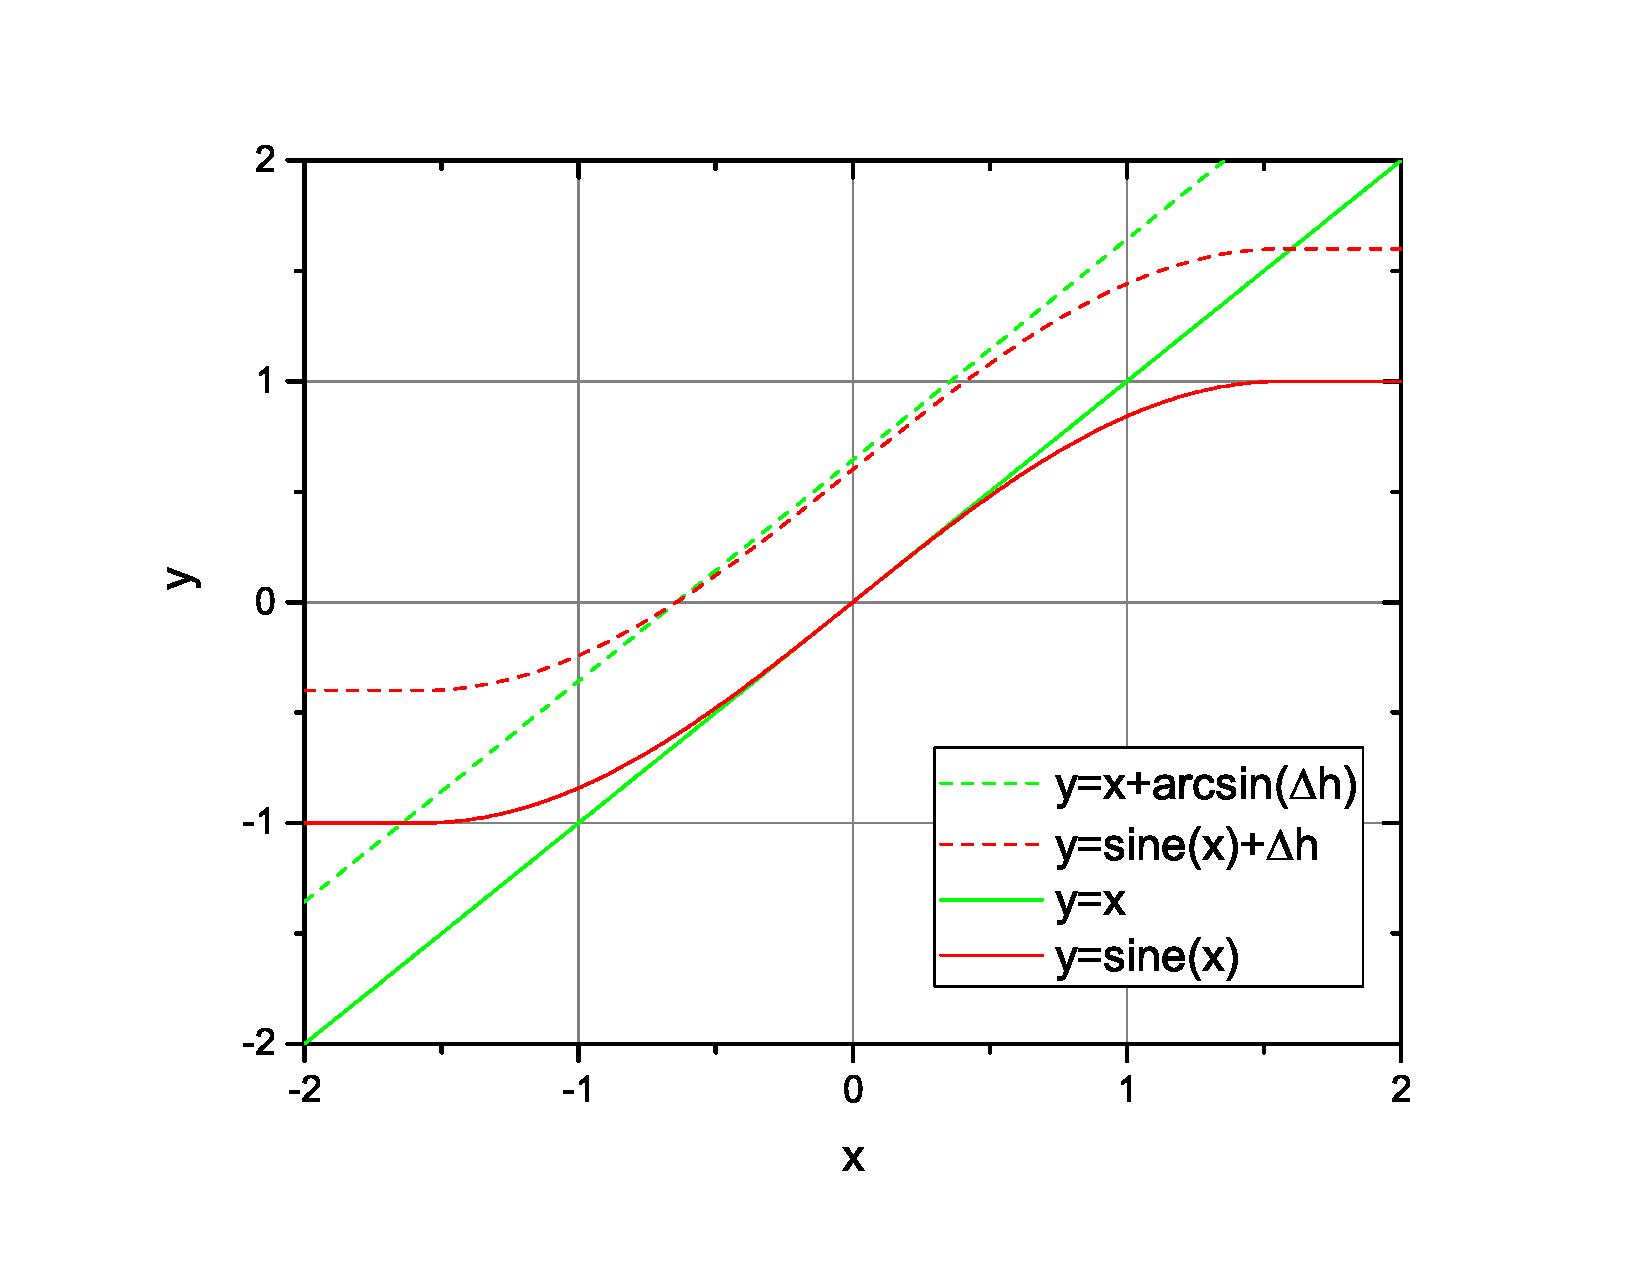
\includegraphics[width=0.75\textwidth]{paper4_fig2.eps}
\caption{$y =Sine(x)$ and $y=Sine(x)+\Delta h$}
\label{fig:2}
\end{figure}
\begin{mylem}\cite{Hu2008552}\label{lemma:2}
Consider a limited function owning the subsequent property:
\begin{align}
g(y) &= R(y)y\in[y_{min},y_{max}]\\
R(y)&=\begin{cases}
y_{max}/y&y>y_{max}\\
1&y_{min}\le y\le y_{max}\\
y_{min}/y&y<y_{min},
\end{cases}
\end{align}
where $y_{min}$ and $y_{max}$ stand for the minimum and maximum values of $g(y)$, respectively, and $y_{min}<0<y_{max}$. If $y$ is bounded, $^by_{min}\le y\le{^by_{max}}$, hence
\begin{align}
0<\min\{y_{min}/{^by_{min}},y_{max}/{^by_{max}}\}\le R(y)\le 1.
\end{align}
\end{mylem}
\begin{myrem}
As we know, \textcolor{red}{the tension, in-plane and out-of-plane thruster force are all limited during deployment mission, and we describe inputs by using the matrix and vector to predigest the following illation.}
\begin{align}
\bm{g}(\tau) &= \left(g(\hat\tau_t),g(\hat\tau_\theta),g(\hat\tau_\phi)\right)^T\\
R_M(\tau) &= \begin{bmatrix}R(\hat\tau_t)&0&0\\0&R(\hat\tau_\theta)&0\\0&0&R(\hat\tau_\phi)\end{bmatrix}.
\end{align}
and in order to design the saturated sliding mode  control for the dynamics of the deployment, the $Sine$ function for vectors is specified as:
\begin{align}
\bm{Sine}(\bm x)=\begin{pmatrix}Sine(x_1),Sine(x_2),\cdots,Sine(x_n)\end{pmatrix}^T.
\end{align}
\end{myrem}
The lemmas above introduce some properties about saturated functions, with which the dynamic sliding mode control subject to input limitation for Lagrangian system~(\ref{eq:dynamic model}) can be designed by using the subsequent theorem.
\begin{mythm}\label{thm:1}(Saturated sliding mode control)
Considering a nominal Lagrangian system~(\ref{eq:dynamic model}) expressing the dynamics of the deployment of the TSS, one can construct a saturated sliding mode control subject to input limitation, as follows:
\begin{align}
\bm\tau = -\bm{g}(\delta\varphi F(t) K_d\bm{sign}(S_{r1})),\label{eq:slider control}
\end{align}
where
\begin{align}
\begin{split}
S_{r1} &= S_{q1}+\gamma\int^t_{t_0}S_{q1}(\varsigma) d\varsigma\\
S_{q1} &= \bm{Sine}(\Delta \dot {\bm q}+\alpha\Delta\bm q),
\end{split}
\end{align}
in which, $F(0)>0$, and the derivative of $F(t)$ has the characteristics:
\begin{align}
\frac{d}{dt}F(t) = \delta\varphi S_{r2}^T K_1K_de^{-2K_1^{-1}F^{-1}(t)}\bm{sign}(S_{r2})
\end{align}
where $K_1\in R^{3\times 3}$ is a positive define diagonal matrix, which will be given out later, and if $K\in R^{3\times 3}$, define
\begin{align}
e^K=
\begin{bmatrix}
e^{K_{11}}&e^{K_{12}}&e^{K_{13}}\\
e^{K_{21}}&e^{K_{22}}&e^{K_{23}}\\
e^{K_{31}}&e^{K_{32}}&e^{K_{33}}
\end{bmatrix}.
\end{align}
\textcolor{red}{$\varphi$ is the boundedness of the lumped uncertainty. $\gamma$ is a small or  time-varying positive scalar, $\varphi>1$ and $K_d$ is the designer parameter, such that the deployment dynamics can be regulated as desired.}
\end{mythm}
\begin{proof}
Consider dynamic coordinates change $S_{r2}$ with the regular error variable but not the $Sine$ form:
\begin{align}
\begin{split}
S_{r2} &= S_{q2}+arcsin(\gamma\int^t_{t_0}S_{q1}(\varsigma) d\varsigma)\\
S_{q2} &= \Delta \dot {\bm q}+\alpha \Delta \bm q,
\end{split}
\end{align}
It is obvious that $S_{q_1}$ is bounded, or exactly saturated, hence $S_{r_1}$ is also bounded if the dynamics can be controlled as desired. In addition, one can select a suitable positive scalar $\gamma$ such that $\gamma\int^t_{t_0}S_{q1}(\varsigma) d\varsigma\in[-1,1]$.\par
According to Lemma~\ref{lemma:1}, it is apparent that $S_{r2}$ and $S_{r1}$ have the subsequent relation:
\begin{align}
&S_{r2}^T \bm{sign}(S_{r2}) \ge  S_{r1}^T \bm{sign}(S_{r1})\\
&\bm{sign}(S_{r2})=\bm{sign}(S_{r1}),
\end{align}
Introducing the limited input~(\ref{eq:slider control}) and replacing the dynamic coordinates change $S_r$ in Eq.~(\ref{eq:dynamic model 2}) with $S_{r2}$ holds results in the following expression:
\begin{align}
H(q)\dot S_{r2} = -\bm{g}(\delta\varphi F(t) K_d\bm{sign}(S_{r1}))-C(q,\dot q)S_{r2}-Y_{r2}\Theta.
\end{align}
Similar to Properties~\ref{pro:1}, one can find a positive scalar $\varphi_2$ such that $\Vert Y_{r2}\Theta\Vert\le\varphi_2$, and moreover the boundedness of the lumped uncertainty $\varphi$ satisfies $\varphi>\varphi_1+\varphi_2$.

Select the Lyapunov function candidate
\begin{align}
V=\frac{1}{2}S_{r2}^TH(q)S_{r2}+\frac{1}{2}v^2,
\end{align}
where $v=F(t)e^{K_1^{-1}F^{-1}(t)}$ and $\frac{1}{2}v^2$ is an auxiliary Lyapunov function with adaptive terms. Differentiating the Lyapunov function above
\begin{align}
\begin{split}
\dot V &= S_{r2}^TH(q)\dot S_{r2}+\frac{1}{2}S_{r2}^T\dot H(q)S_{r2}+v\dot v\\
&= -S_{r2}^T\bm{g}(\delta\varphi F(t) K_d\bm{sign}(S_{r1}))+S_{r2}^T\bm\tau_d-S_{r2}^TC(q,\dot q)S_{r2}+\frac{1}{2}S_{r2}^T\dot H(q)S_{r2}-S_{r2}^TY_{r2}\Theta+v\dot v\\
&= -S_{r2}^T\bm{g}(\delta\varphi F(t) K_d\bm{sign}(S_{r1}))+S_{r2}^T\bm\tau_d-S_{r2}^TY_{r2}\Theta+\frac{1}{2}S_{r2}^T(\dot H(q)-2C(q,\dot q))S_{r2}+v\dot v\\
&= -S_{r2}^T\bm{g}(\delta\varphi F(t) K_d\bm{sign}(S_{r1}))+S_{r2}^T\bm\tau_d-S_{r2}^TY_{r2}\Theta+v\dot v\\
&= -S_{r2}^TR_M(\delta\varphi F(t) K_d\bm{sign}(S_{r1}))\delta\varphi F(t) K_d\bm{sign}(S_{r1})+S_{r2}^T\bm\tau_d-S_{r2}^TY_{r2}\Theta+v\dot v.\label{eq:V1_1}
\end{split}
\end{align}
Since the command $ -\delta\varphi F(t) K_dS_{r1}$ is bounded, one can select reasonably small positive scalars $c_1$ and $c_2$ such that $0<c_1\le R(\hat\tau_t)<1$ and $0<c_2\le R(\hat\tau_\theta)<1$, and obtain a diagonal matrix as follows:
\begin{align}
K_1 = \begin{bmatrix}c_1&0\\0&c_2\end{bmatrix}.\label{eq:saturated ratio}
\end{align}
$v\dot v$ is able to be derived as follows:
\begin{align}
v\dot v =\varphi\delta S_{r2}^T K_1K_d(F(t)-K_1^{-1})\bm{sign}(S_{r2}),
\end{align}
utilizing $\bm{sign}(S_{r1})=\bm{sign}(S_{r2})$ and $K_1$ proceeds to rewrite Eq.~(\ref{eq:V1_1}) as:
\begin{align}
\begin{split}\label{eq:V1_2}
\dot V&\le -S_{r2}^T\delta\varphi  K_1K_dF(t)\bm{sign}(S_{r2})+S_{r2}^T(\varphi_1+\varphi_2) \bm{sign}(S_{r2})+\varphi\delta S_{r2}^T K_1K_d(F(t)-K_1^{-1})\bm{sign}(S_{r2})\\
&\le \varphi S_{r2}^T\bm{sign}(S_{r2})-\varphi\delta S_{r2}^T K_d\bm{sign}(S_{r2})
\end{split}
\end{align}
owing to the boundedness of the expression above, a large enough $\delta$ can be selected such that $\dot V \le 0$. According to the description of Barbalat��s lemmas, it implies that $S_{r2}$ asymptotically converges to zero with the set of suitable designer parameters.\par
Utilizing $S_{r2}=0$ leads to the equation
\begin{align}
S_{q2}=-arcsin(\gamma\int^t_{t_0}S_{q1}(\varsigma) d\varsigma),\label{eq:eqSq2}
\end{align}
and select a Lyapunov function candidate
\begin{align}
V_1 = \frac{1}{2}S_{q2}^TS_{q_2},
\end{align}
the derivative of which gives rise to
\begin{align}
\begin{split}
\dot V_1 &= S_{q2}^T\dot S_{q_2}\\
&=-\frac{\gamma S_{q2}^TS_{q1}}{\sqrt{1-\Vert\gamma\int^t_{t_0}S_{q1}(\varsigma) d\varsigma\Vert^2}}\\
&\le -\frac{\gamma \Vert S_{q1}\Vert^2}{\sqrt{1-\Vert\gamma\int^t_{t_0}S_{q1}(\varsigma) d\varsigma\Vert^2}}\le 0,
\end{split}
\end{align}
if and only if $S_{q1} = 0$, accordingly, $S_{q2} = 0$, one has $\dot V_1=0$. Hence the asymptotically stability of Eq.~(\ref{eq:eqSq2}) has been proved, and therefore $S_{q2}\rightarrow 0$ as $t\rightarrow \infty$ produces
\begin{align}
\Delta \dot {\bm q}=-\alpha \Delta \bm q.
\end{align}
Select the Lyapunov function candidate $V_2=\frac{1}{2}\Delta \bm q^T\Delta\bm q$, the derivative of which follows
\begin{align}
\begin{split}
\dot V_2 &= \Delta\bm q^T\Delta \dot{\bm q}\\
&=-\alpha \Delta \bm q^T\Delta \bm q\le 0,
\end{split}
\end{align}
if and only if $\Delta \bm q = 0$, namely, $\Delta \dot {\bm q} = 0$, one has $\dot V_2=0$. Hence asymptotically convergence of $\Delta \bm q$ has been explained, namely, $\Delta \bm q\rightarrow 0$ as $t\rightarrow \infty$. To conclude, the error state $\Delta \bm q$ of the system~(\ref{eq:dynamics 1}) asymptotically converges to the origin with the limited input~(\ref{eq:slider control}). This completes the proof.
\end{proof}
\subsection{Quasi-saturated terminal sliding mode control subject to input limitation}
The design methodology of the saturated sliding mode control has been exhibited in last subsection, and the entire strict proof ensures that the dynamics of the deployment of the tethered satellite can be regulated with the limited tension control. Essentially, the method mentioned above is able to perform a limited sliding mode controller, since the order of the integrated error is one. If the order of the integrated error varies to become a fraction, the value of which is less than one, one establishes the terminal attractor like
\begin{align}
\dot Z = Z^{p/q},
\end{align}
where $0<p/q<1$ and $p$ and $q$ are both positive odd, and a shrewd formula
\begin{align}
\dot Z = \vert Z\vert^{\hat\alpha} \bm{sign}(Z),
\end{align}
where $0<\hat \alpha<1$, performs the same behavior. Inducting the terminal attractor into the saturated sliding mode control yields a saturated slider-like scheme, and for adopting to the system subject to input limitation, an assumption is given firstly.
\begin{myas}\label{as:1}
For Eq.~(\ref{eq:dynamic model}), the length rate is thought to be bounded during the deployment, namely, $0<\epsilon\le\dot \lambda<\infty$, such that $\Delta \dot \lambda$ is bounded, either.
\end{myas}
\begin{mythm}\label{thm:2}(Quasi-saturated terminal sliding mode control)
Considering the dynamics of the deployment as described in Eq.~(\ref{eq:dynamic model}) with limited tension control, the quasi-saturated terminal sliding mode control input can be designed as follow:
\begin{align}
\tau = -\bm{g}(\delta\varphi F(t) K_{d1}\bm{sign}(S_{r3}))
\end{align}
where
\begin{align}
S_{r3} &= S_{q3}+\gamma\int^t_{t_0}\Vert S_{q3}(\varsigma)\Vert^{\hat\alpha}  \bm{sign}(S_{q3}(\varsigma))d\varsigma\label{eq:Sr3}\\
S_{q3} &= \Delta \dot q+\alpha \bm{Sine}(\xi\Delta q),\label{eq:Sq3}
\end{align}
where $0<\hat\alpha< 1$, such that the dynamics~(\ref{eq:dynamic model 2}) can be regulated as desired. $\varphi$ is the boundedness of the lumped uncertainty, and can be obtained by referring to Theorem~\ref{thm:1}.
\end{mythm}
\begin{proof}
The proof is similar to Theorem~\ref{thm:1}, and omitted here.
\end{proof}
\begin{myrem}
If the designer parameter $\hat\alpha = 1$, the quasi-saturated terminal sliding mode control degenerates into the quasi-saturated sliding mode control. Compared with the saturated sliding mode control, $S_{q3}$ converges to the origin in finite time in the quasi-saturated terminal method. This is because the establishment of the equation $\dot S_{q3} = \gamma\Vert S_{q3}\Vert^{\hat\alpha} \bm{ sign}(S_{q3})$.
\end{myrem}
\begin{myrem}
Assumption~\ref{as:1} guarantees that the input $\tau$ is bounded in Theorem~\ref{thm:2}, accordingly, a tiny positive scalar $c$ is able to be found such that $0<c\le R(\hat\tau_t)<1$ always exists. Admittedly, such kind of assumption is ''skillful'', but meaningful to arbitrary controllable dynamics in reality. It is reasonable to propose the terminal sliding mode control for the dynamics as follows:
\begin{align}
\tau = -\bm{g}(\delta\varphi F(t) K_{d1}\bm{sign}(S_{r4})),
\end{align}
where
\begin{align}
\begin{split}
S_{r4} &= S_{q4}+\gamma\int^t_{t_0}S_{q4}(\varsigma) d\varsigma\\
S_{q4} &= \bm{Sine}(\Delta \dot q+\alpha\xi\Vert\Delta q\Vert^{\hat\alpha}\bm{sign}(\Delta q)),\label{eq:Sr4}
\end{split}
\end{align}
such that the finite convergence of the system~(\ref{eq:Sr4}) can be ensured by using terminal sliding mode theory. $\varphi$ is the boundedness of the lumped uncertainty, and can be obtained by referring to Theorem~\ref{thm:1}.
\end{myrem}
\section{Simulation studies}\label{sec:4}
In this section, the simulations of the regulation of the deployment dynamics with saturated sliding mode control, saturated terminal sliding mode control and quasi-saturated terminal sliding mode control, and for clarity, these controllers are abbreviated as S-SMC, ST-SMC and QSF-SMC, respectively. The parameters of these controllers can selected as follows: $\delta=1.1$, $\varphi= 1\times 10^{-3}$, $\alpha = 0.8$, $K_d(K_{*})=1$, $\gamma = 0.1$ and $\hat\alpha=0.6$.\par
Besides the designer parameter determined, the simulation initial and desired condition can be described as follows. The circular orbital altitude is selected around 260 $km$ approximately, and the orbital angular velocity is about $1.17\times 10^{-3}$ $rad/s$. At the initial ejection of the subsatellite, the true anomaly is assumed 0 $rad$. Meanwhile, the initial deployment velocity is about 3 $m/s$, and the subsatellite is going to be deployed at 3.5 $km$ vertically. The pitching and rolling dynamics is varying in a small range, and hence, without loss of generality, the numerical initial condition gives rise to: $\theta_0 = 0.1$, $\varphi_0 = 0.1$, $\lambda_0 = 0.02$; the desired condition is set to be $\theta_d = 0$, $\phi_d = 0$ and $\lambda_d = 1$, accordingly, $\lambda(t_0)\rightarrow\lambda_d$, $t\rightarrow\infty$ with $\theta(t_0)\rightarrow\theta_d$, $\phi(t_0)\rightarrow\phi_d$, $t\rightarrow\infty$. Hence the dimensionless tether length is varying in $[0.02,1]$.\par
During the deployment, the dimensionless thruster forces which manage the in-plane angle and the out-of-plane angle are assumed to be saturated with $\vert\hat\tau_{\theta}\vert\le5 $ and $\vert\hat\tau_{\phi}\vert\le 5$. Also, the dimensionless tension $\hat\tau_t$ is limited, and from Eq.~(\ref{eq:varcon}), one can obtain
\begin{align}
\begin{split}
&0<\tau_{tmin}/(\bar{m}\Omega^2L)\le-\hat\tau_t+\lambda\le\tau_{tmax}/(\bar{m}\Omega^2L)\\
\Leftrightarrow
&\begin{cases}
\max\{-\hat\tau_t+\lambda\}\le\tau_{tmax}/(\bar{m}\Omega^2L)\\
\min\{-\hat\tau_t+\lambda\}\ge\tau_{tmin}/(\bar{m}\Omega^2L)
\end{cases}\\
\Leftrightarrow
&\begin{cases}
-\hat\tau_{tmin}+\lambda_{max}\le\tau_{tmax}/(\bar{m}\Omega^2L)\\
-\hat\tau_{tmax}+\lambda_{min}\ge\tau_{tmin}/(\bar{m}\Omega^2L).
\end{cases}
\end{split}
\end{align}
Hence, the limited dimensionless tension gives rise to
\begin{align}
-\tau_{tmax}/(\bar{m}\Omega^2L)+\lambda_{max}\le\hat\tau_{tmin}\le\hat\tau_t\le\hat\tau_{tmax}\le-\tau_{tmin}/(\bar{m}\Omega^2L)+\lambda_{min}.
\end{align}
Based on the expression above, one can obtain $\bar{m}\Omega^2L\approx 4.79\times 10^{-3}$, and suitable bounded values $\hat\tau_{tmin}$ and $\hat\tau_{tmax}$ can be chosen to make the dimensionless tension $\hat\tau_t$ fall in the region $[-3,0.01]$.\par
At this point, the simulations of the deployment dynamics of the TSS are able to be carried on, and the results are illustrated in Figure~\ref{fig:3} to~\ref{fig:6}. Figure~\ref{fig:3} shows the dynamics of the length in different control laws, and it is obvious that the all the methods finish the deployment in aspect of the tether length. ST-SMC and QST-SMC complete the deployment at about 4 $rad$, and from Figure~\ref{fig:4}, S-SMC and QST-SMC have bigger length rate than ST-SMC before 1.2 $rad$, and hence the curves of the tether length climb more rapidly at the beginning. In contrary, the length rate of ST-SMC doesn't decline dramatically like the other two methods after 1.2 $rad$. This slowly varying length rate yields a smooth trajectory of the deployment shown in Figure~\ref{fig:3}, and meanwhile the length rate converges to origin more early than $S-SMC$ and $QST-SMC$.\par
The in-plane and out-of-plane angles reflect the swinging dynamics of the tether during the deployment, the details of which are drawn in Figue~\ref{fig:5}. For ST-SMC, the in-plane dynamics is regulated to vertical status at 4 $rad$, and the in-plane angle converges to the origin in the subsequent time, and hence the coalition of the length and the swinging dynamics implies that the whole deployment mission is completed at about 4 $rad$ by utilizing ST-SMC. S-SMC makes the tether swing to desired position at a low convergent speed near the vertical direction during 2 $rad$ to 4 $rad$.\par
The inputs in S-SMC for dynamic model~(\ref{eq:dynamic model}) is exhibited in Figure~\ref{fig:6}, in which it is obvious that the limited situations occur frequently. Thanks to the scalable dimensionless transform determined conservatively, the tension exerted on the tether falls in the reasonable region.
\begin{figure}
\centering
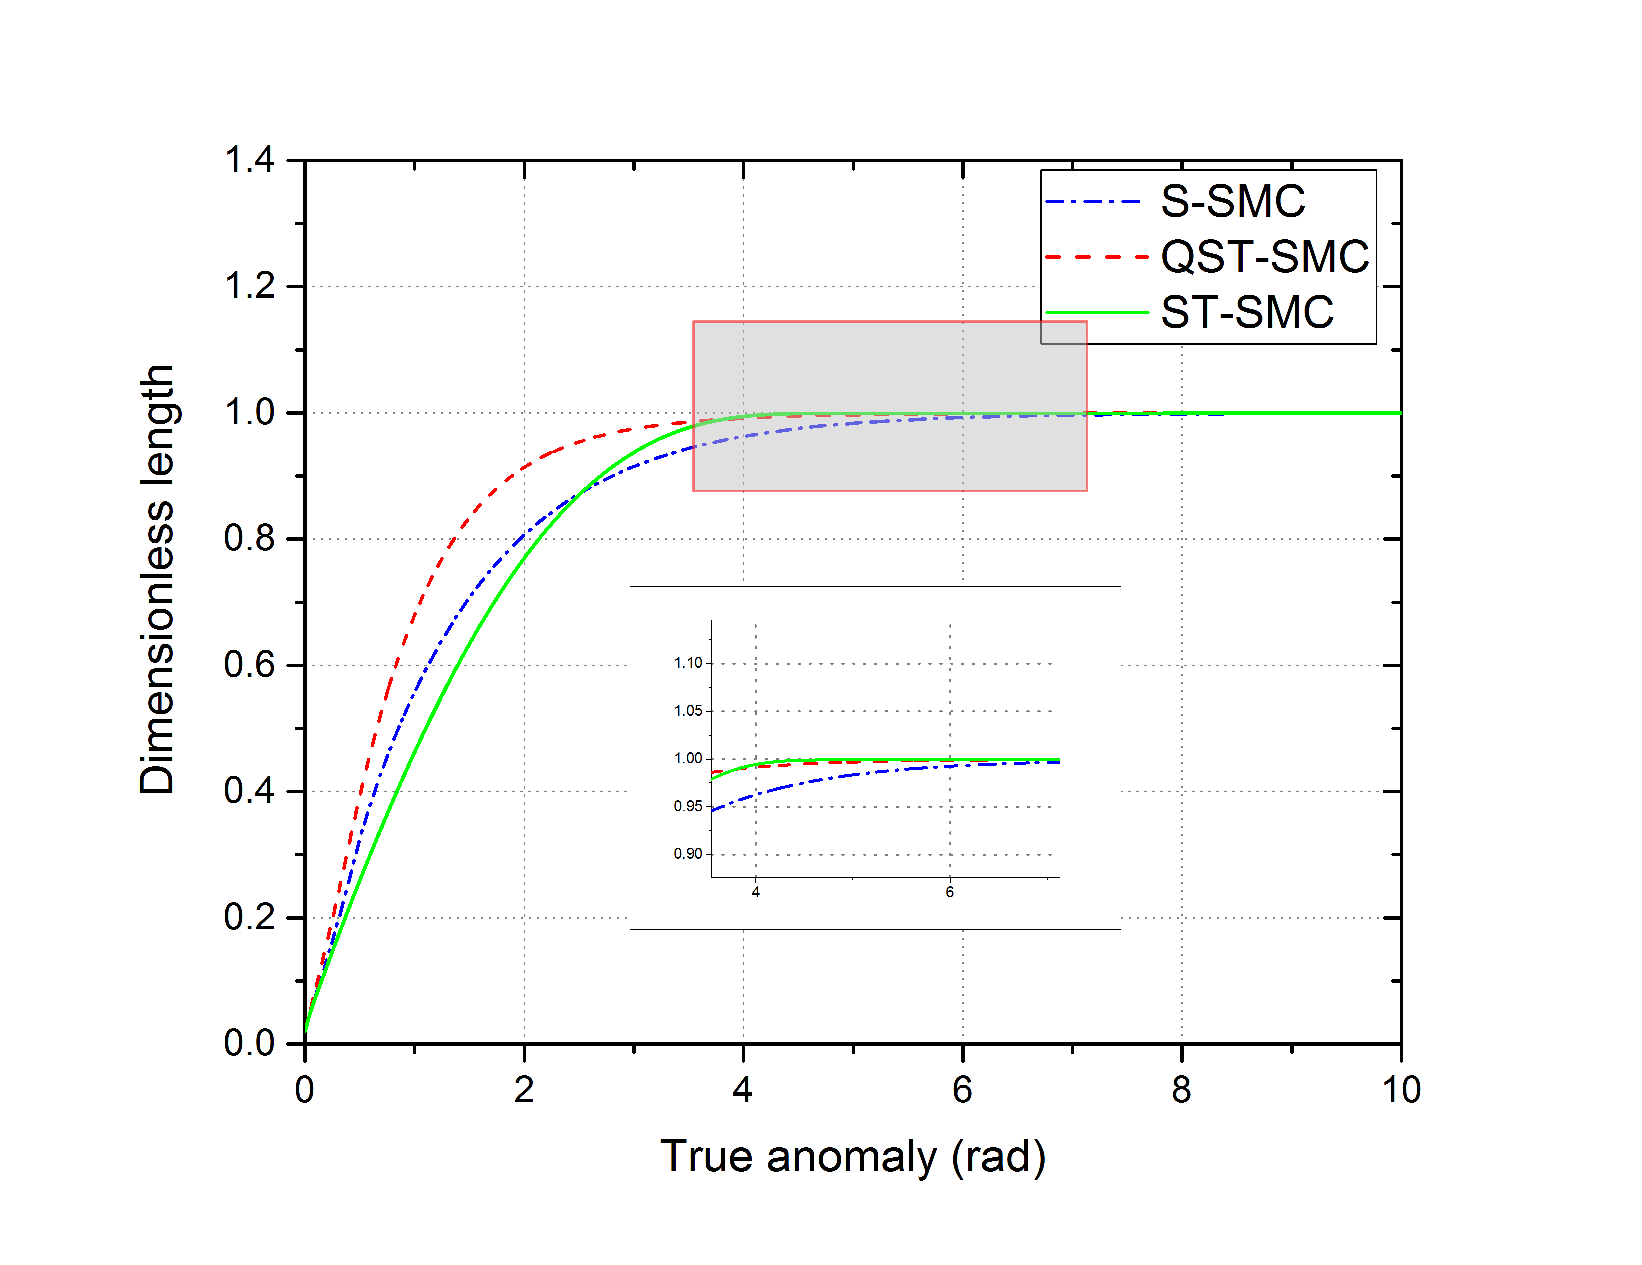
\includegraphics[width=0.6\textwidth]{paper4_fig3.eps}
\caption{Length dynamics of the deployment}
\label{fig:3}
\end{figure}
\begin{figure}
\centering
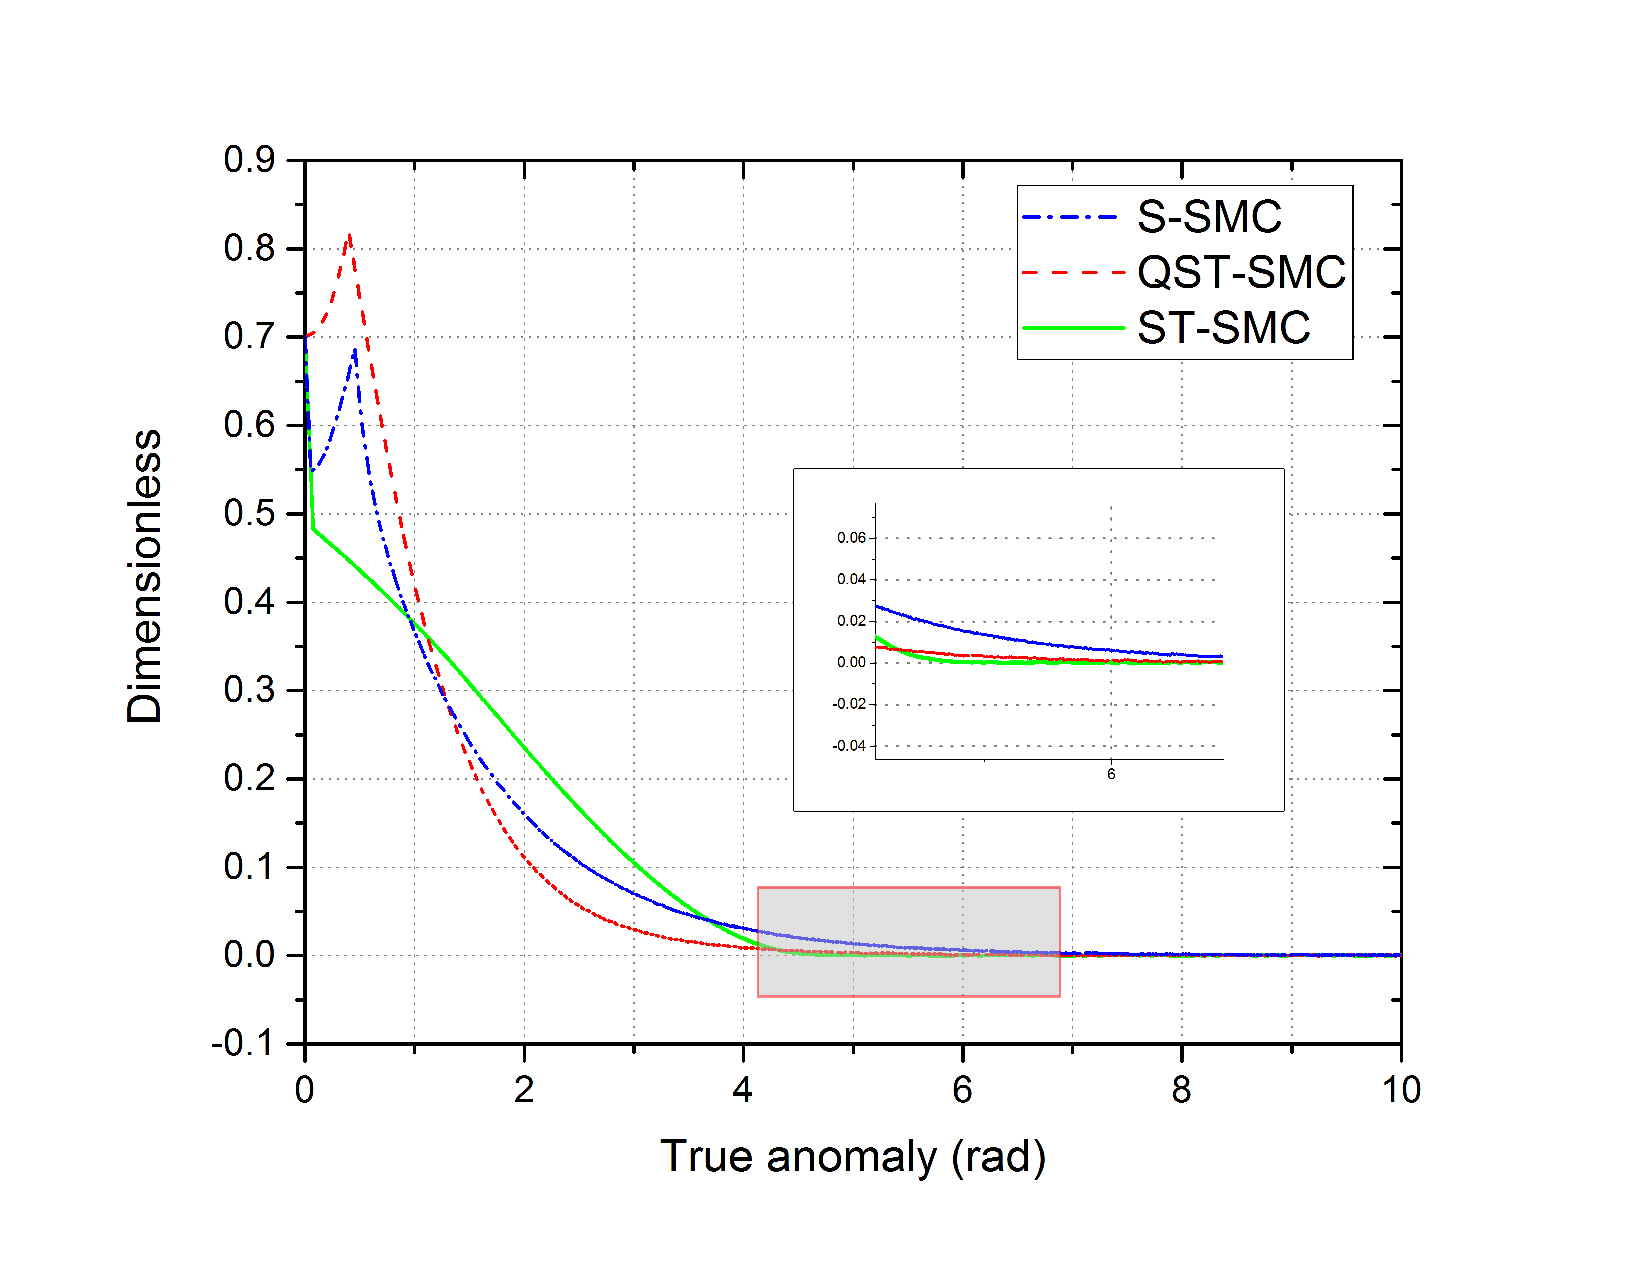
\includegraphics[width=0.6\textwidth]{paper4_fig4.eps}
\caption{Length rate dynamics of the deployment}
\label{fig:4}
\end{figure}
\begin{figure}
\centering
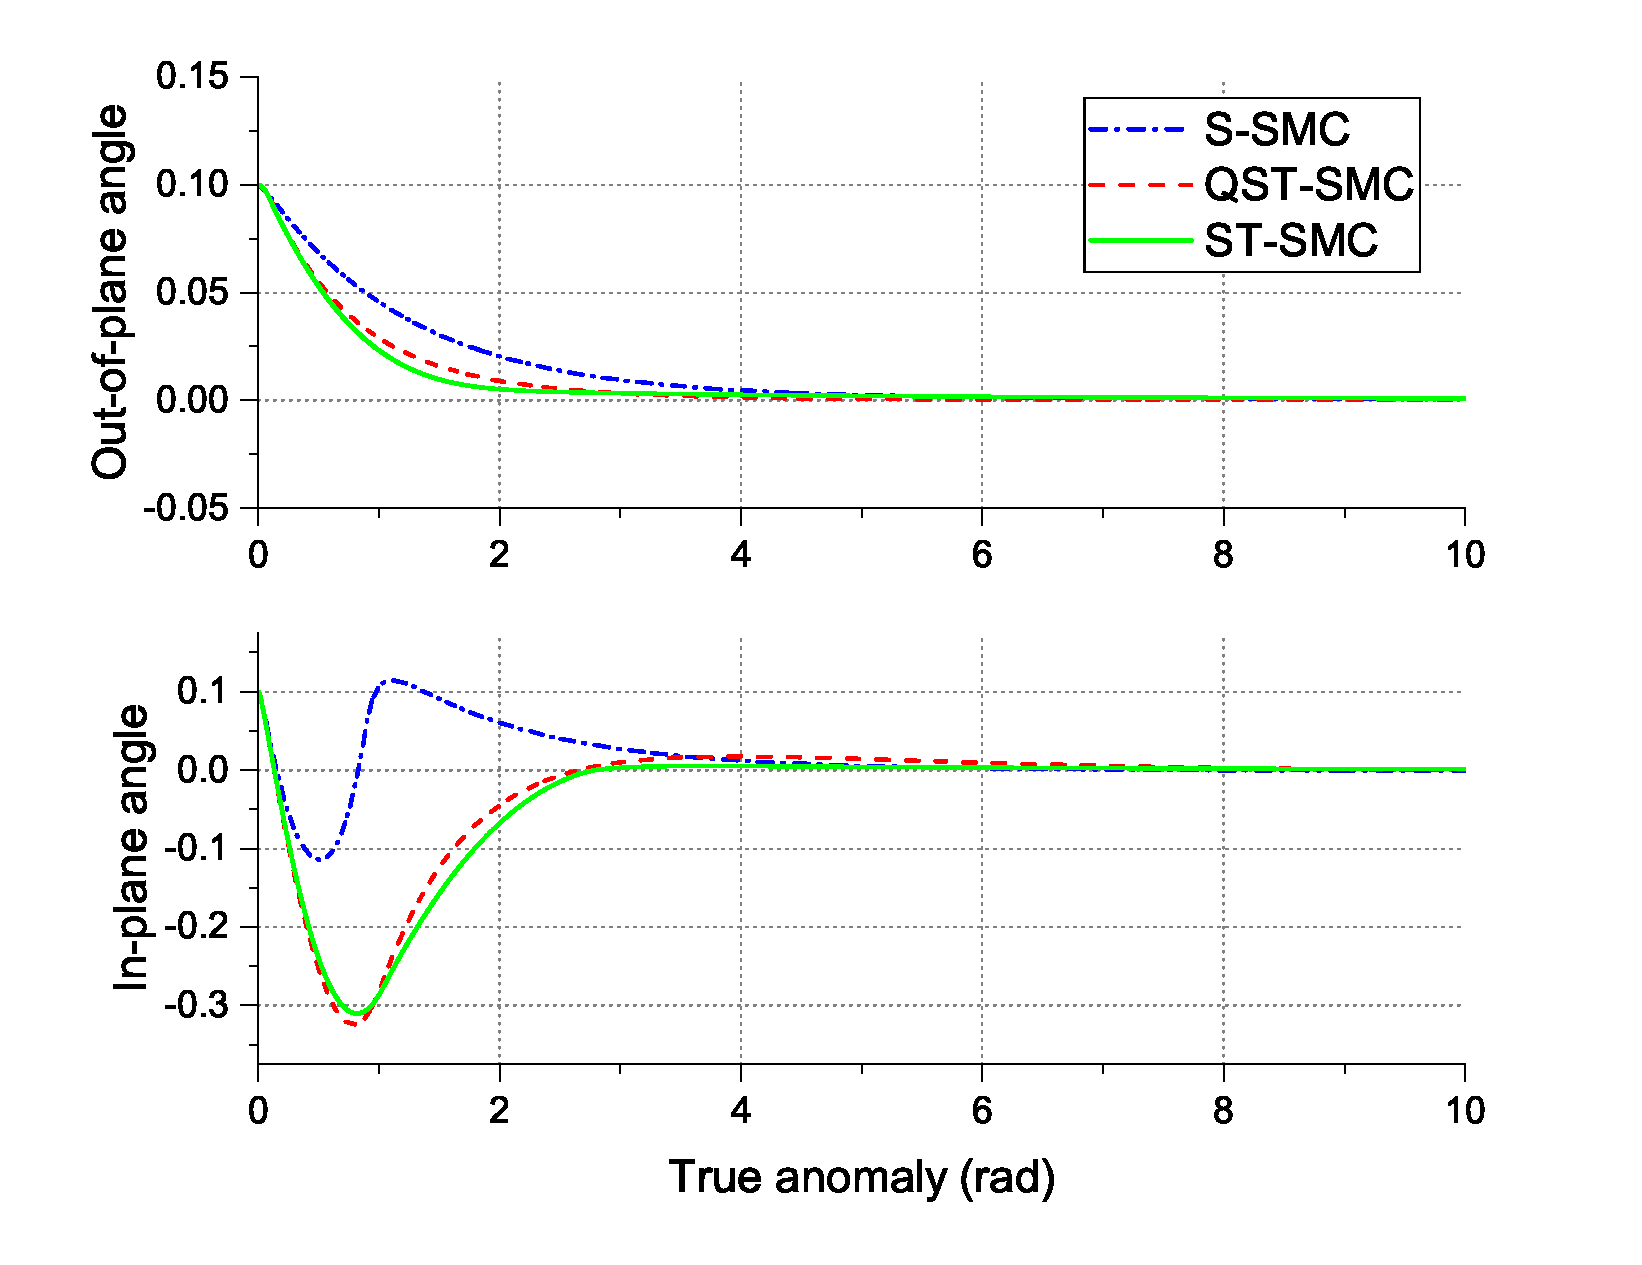
\includegraphics[width=0.6\textwidth]{paper4_fig5.eps}
\caption{Angle dynamics of the deployment}
\label{fig:5}
\end{figure}
\begin{figure}
\centering
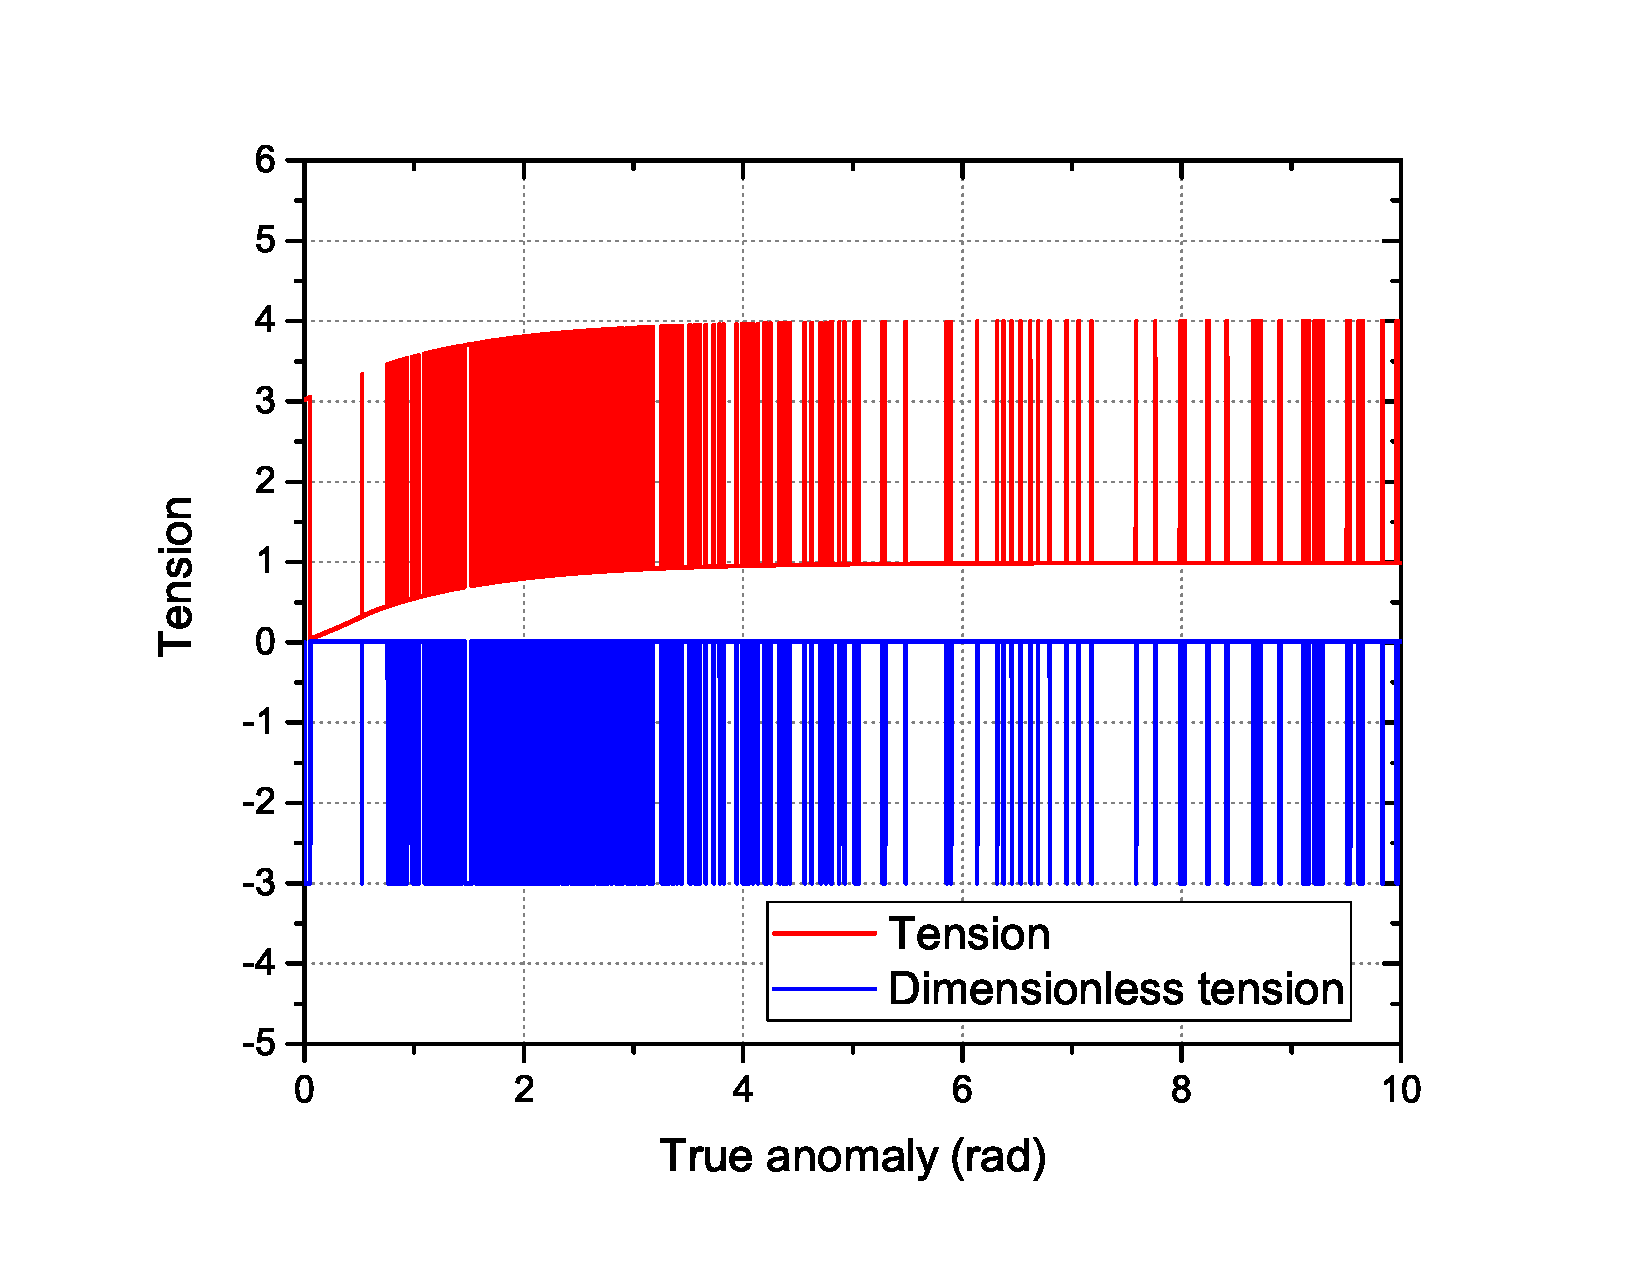
\includegraphics[width=0.6\textwidth]{paper4_fig6.eps}
\caption{Tension}
\label{fig:6}
\end{figure}
\section{Conclusion}\label{sec:5}
In this paper, the error dynamics of the deployment of the TSS provides the adaptive sliding mode control with a simplified solution for the reaching phase, which ignores the nonlinear nature of the model, and the new dimensionless transformation subject to the limited input guarantees the effectiveness of the auxiliary Lyapunov function with adaptive terms. The simulation results show that the proposed methods adjust the length of the tether and the swinging dynamics as desired, although there exists the input limitation during the deployment. According to the results mentioned above, combining error dynamics design approach, adaptive approach and nonlinear sliding mode surface design technology may provide a further insight into regulation of the dynamics of the deployment of the tethered satellite system.
\section{Acknowledgment}
This work is partially supported by the National Natural Science Foundation of China (No. 61104112, 61503101).
\section{References}
\bibliography{paper4_ref}
\bibliographystyle{elsarticle-num}
\end{document}


